% Options for packages loaded elsewhere
\PassOptionsToPackage{unicode}{hyperref}
\PassOptionsToPackage{hyphens}{url}
\PassOptionsToPackage{dvipsnames,svgnames,x11names}{xcolor}
%
\documentclass[
  letterpaper,
  DIV=11,
  numbers=noendperiod]{scrartcl}

\usepackage{amsmath,amssymb}
\usepackage{iftex}
\ifPDFTeX
  \usepackage[T1]{fontenc}
  \usepackage[utf8]{inputenc}
  \usepackage{textcomp} % provide euro and other symbols
\else % if luatex or xetex
  \usepackage{unicode-math}
  \defaultfontfeatures{Scale=MatchLowercase}
  \defaultfontfeatures[\rmfamily]{Ligatures=TeX,Scale=1}
\fi
\usepackage{lmodern}
\ifPDFTeX\else  
    % xetex/luatex font selection
\fi
% Use upquote if available, for straight quotes in verbatim environments
\IfFileExists{upquote.sty}{\usepackage{upquote}}{}
\IfFileExists{microtype.sty}{% use microtype if available
  \usepackage[]{microtype}
  \UseMicrotypeSet[protrusion]{basicmath} % disable protrusion for tt fonts
}{}
\makeatletter
\@ifundefined{KOMAClassName}{% if non-KOMA class
  \IfFileExists{parskip.sty}{%
    \usepackage{parskip}
  }{% else
    \setlength{\parindent}{0pt}
    \setlength{\parskip}{6pt plus 2pt minus 1pt}}
}{% if KOMA class
  \KOMAoptions{parskip=half}}
\makeatother
\usepackage{xcolor}
\setlength{\emergencystretch}{3em} % prevent overfull lines
\setcounter{secnumdepth}{5}
% Make \paragraph and \subparagraph free-standing
\ifx\paragraph\undefined\else
  \let\oldparagraph\paragraph
  \renewcommand{\paragraph}[1]{\oldparagraph{#1}\mbox{}}
\fi
\ifx\subparagraph\undefined\else
  \let\oldsubparagraph\subparagraph
  \renewcommand{\subparagraph}[1]{\oldsubparagraph{#1}\mbox{}}
\fi


\providecommand{\tightlist}{%
  \setlength{\itemsep}{0pt}\setlength{\parskip}{0pt}}\usepackage{longtable,booktabs,array}
\usepackage{calc} % for calculating minipage widths
% Correct order of tables after \paragraph or \subparagraph
\usepackage{etoolbox}
\makeatletter
\patchcmd\longtable{\par}{\if@noskipsec\mbox{}\fi\par}{}{}
\makeatother
% Allow footnotes in longtable head/foot
\IfFileExists{footnotehyper.sty}{\usepackage{footnotehyper}}{\usepackage{footnote}}
\makesavenoteenv{longtable}
\usepackage{graphicx}
\makeatletter
\def\maxwidth{\ifdim\Gin@nat@width>\linewidth\linewidth\else\Gin@nat@width\fi}
\def\maxheight{\ifdim\Gin@nat@height>\textheight\textheight\else\Gin@nat@height\fi}
\makeatother
% Scale images if necessary, so that they will not overflow the page
% margins by default, and it is still possible to overwrite the defaults
% using explicit options in \includegraphics[width, height, ...]{}
\setkeys{Gin}{width=\maxwidth,height=\maxheight,keepaspectratio}
% Set default figure placement to htbp
\makeatletter
\def\fps@figure{htbp}
\makeatother
\newlength{\cslhangindent}
\setlength{\cslhangindent}{1.5em}
\newlength{\csllabelwidth}
\setlength{\csllabelwidth}{3em}
\newlength{\cslentryspacingunit} % times entry-spacing
\setlength{\cslentryspacingunit}{\parskip}
\newenvironment{CSLReferences}[2] % #1 hanging-ident, #2 entry spacing
 {% don't indent paragraphs
  \setlength{\parindent}{0pt}
  % turn on hanging indent if param 1 is 1
  \ifodd #1
  \let\oldpar\par
  \def\par{\hangindent=\cslhangindent\oldpar}
  \fi
  % set entry spacing
  \setlength{\parskip}{#2\cslentryspacingunit}
 }%
 {}
\usepackage{calc}
\newcommand{\CSLBlock}[1]{#1\hfill\break}
\newcommand{\CSLLeftMargin}[1]{\parbox[t]{\csllabelwidth}{#1}}
\newcommand{\CSLRightInline}[1]{\parbox[t]{\linewidth - \csllabelwidth}{#1}\break}
\newcommand{\CSLIndent}[1]{\hspace{\cslhangindent}#1}

\usepackage{booktabs}
\usepackage{longtable}
\usepackage{array}
\usepackage{multirow}
\usepackage{wrapfig}
\usepackage{float}
\usepackage{colortbl}
\usepackage{pdflscape}
\usepackage{tabu}
\usepackage{threeparttable}
\usepackage{threeparttablex}
\usepackage[normalem]{ulem}
\usepackage{makecell}
\usepackage{xcolor}
\addtokomafont{disposition}{\rmfamily}
\KOMAoption{captions}{tableheading}
\makeatletter
\makeatother
\makeatletter
\makeatother
\makeatletter
\@ifpackageloaded{caption}{}{\usepackage{caption}}
\AtBeginDocument{%
\ifdefined\contentsname
  \renewcommand*\contentsname{Table of contents}
\else
  \newcommand\contentsname{Table of contents}
\fi
\ifdefined\listfigurename
  \renewcommand*\listfigurename{List of Figures}
\else
  \newcommand\listfigurename{List of Figures}
\fi
\ifdefined\listtablename
  \renewcommand*\listtablename{List of Tables}
\else
  \newcommand\listtablename{List of Tables}
\fi
\ifdefined\figurename
  \renewcommand*\figurename{Figure}
\else
  \newcommand\figurename{Figure}
\fi
\ifdefined\tablename
  \renewcommand*\tablename{Table}
\else
  \newcommand\tablename{Table}
\fi
}
\@ifpackageloaded{float}{}{\usepackage{float}}
\floatstyle{ruled}
\@ifundefined{c@chapter}{\newfloat{codelisting}{h}{lop}}{\newfloat{codelisting}{h}{lop}[chapter]}
\floatname{codelisting}{Listing}
\newcommand*\listoflistings{\listof{codelisting}{List of Listings}}
\makeatother
\makeatletter
\@ifpackageloaded{caption}{}{\usepackage{caption}}
\@ifpackageloaded{subcaption}{}{\usepackage{subcaption}}
\makeatother
\makeatletter
\@ifpackageloaded{tcolorbox}{}{\usepackage[skins,breakable]{tcolorbox}}
\makeatother
\makeatletter
\@ifundefined{shadecolor}{\definecolor{shadecolor}{rgb}{.97, .97, .97}}
\makeatother
\makeatletter
\makeatother
\makeatletter
\makeatother
\ifLuaTeX
  \usepackage{selnolig}  % disable illegal ligatures
\fi
\IfFileExists{bookmark.sty}{\usepackage{bookmark}}{\usepackage{hyperref}}
\IfFileExists{xurl.sty}{\usepackage{xurl}}{} % add URL line breaks if available
\urlstyle{same} % disable monospaced font for URLs
\hypersetup{
  pdftitle={Finding suitable weather indices for novel fisheries index insurance using machine learning},
  pdfauthor={Nathaniel Grimes},
  pdfkeywords={Index Insurance, Fisheries, Machine Learning},
  colorlinks=true,
  linkcolor={blue},
  filecolor={Maroon},
  citecolor={Blue},
  urlcolor={Blue},
  pdfcreator={LaTeX via pandoc}}

\title{Finding suitable weather indices for novel fisheries index
insurance using machine learning}
\usepackage{etoolbox}
\makeatletter
\providecommand{\subtitle}[1]{% add subtitle to \maketitle
  \apptocmd{\@title}{\par {\large #1 \par}}{}{}
}
\makeatother
\subtitle{Working Paper not for Distribution}
\author{Nathaniel Grimes}
\date{2024-11-26}

\begin{document}
\maketitle
\begin{abstract}
Index insurance is a financial tool gaining traction for application in
fisheries. It will cover fishers losses under extreme weather events
that impact fishery productivity. This is the first assessment to
determine the feasibility of such programs and whether suitable indices
exist. Catch and revenue data from 74 California fisheries are matched
to 20 environmental variables using three prediction models: linear
regression, LASSO regression, and random forests. The models are used to
calculate the maringal willingness to pay through utility models.
\end{abstract}
\ifdefined\Shaded\renewenvironment{Shaded}{\begin{tcolorbox}[frame hidden, boxrule=0pt, enhanced, interior hidden, borderline west={3pt}{0pt}{shadecolor}, breakable, sharp corners]}{\end{tcolorbox}}\fi

\renewcommand*\contentsname{Table of contents}
{
\hypersetup{linkcolor=}
\setcounter{tocdepth}{3}
\tableofcontents
}
\hypertarget{introduction}{%
\section{Introduction}\label{introduction}}

Predicting fishery output from weather variables is notoriously
difficult. It is widely established that climate and weather affect
fishing populations (Lehodey \emph{et al.} 2006), but most stock
assessment models use little to no year to year environmental data
(Privitera-Johnson and Punt 2020). Variations in environmental
conditions are now the leading cause of fishery closures and disaster
relief payouts in the United States (Bellquist \emph{et al.} 2021).
Disaster declarations are becoming more frequent straining a slow,
inequitable system (Holland and Leonard 2020; Jardine \emph{et al.}
2020). Calls for new financial tools to alleviate fisher income shocks
have grown (Mumford \emph{et al.} 2009; Sethi 2010).

Index insurance has risen as a prime candidate to protect fishing
communities during disasters (Watson \emph{et al.} 2023). Index
insurance is a financial product that pays out when an independently
verified index, such as rainfall or temperature, falls below a
predetermined threshold. The index is chosen to be highly correlated
with the asset being insured. However, it is difficult to establish
clear, concise weather impacts on fishery productivity. The biological
dynamics of the system can lead to lower stock health persisting for
years after a negative shock (Hilborn \emph{et al.} 2003). Individual
fisheries can cover enormous areas in ocean basins. The expansive
spatial coverage of fisheries makes it unclear where and how much
specific weather variables impact biological abundance. In addition, if
weather impacts have been observed, they are most likely highly
non-linear adding further complexity. The greatest impediment to the
development of fishery insurance policies is reconciling these
challenges to find suitable indices that can predict fishery
productivity (Watson \emph{et al.} 2023).

The difficulty in modelling fishery productivity with environmental
indices leads to basis risk. Formally, basis risk is the probability
that policyholders experience a harmful shock to their income, but the
index does not trigger. Basis risk lowers demand for index insurance and
remains a significant roadblock in setting up new programs
(Binswanger-Mkhize 2012; Clarke 2016; Clement \emph{et al.} 2018).

It is impossible to completely eliminate basis risk. Well designed
policies can capture up to 90\% of the income variation as shown in
Kenyan pasture grazing indices (Jensen \emph{et al.} 2019). Abysmal
correlations are prevalent in the Rainfall Index Insurance for Pasture,
Rangeland, and Forage (RI-PRF) program where correlations as low as
0.071 exist in California, which leads to 46\% additional points of
basis risk (Keller and Saitone 2022). The program has a 26\% probability
of not paying out when damages are suffered in Nebraska and Kansas (Yu
\emph{et al.} 2019). Subsidies covering up to 60\% of ranchers paid
premiums are needed to stimulate demand in the RI-PRF program (Goodrich
\emph{et al.} 2019).

Designing indices with stronger correlations to fishery losses is the
most effective way to reduce basis risk (Jensen \emph{et al.} 2019).
Agricultural researchers continually seek new methods and data sources
to improve the correlation between loss and weather variables. Quantile
regressions improve Kazak wheat farmers utility between 0.1-22\% over
linear models depending on the underlying measure of utility (Conradt
\emph{et al.} 2015). Remote sensing variables leveraging the latest
satellite data on vegetative cover and rainfall provide better coverage
than county wide averages (Dalhaus and Finger 2016; Valverde-Arias
\emph{et al.} 2020).

Machine learning has exploded as a new method to define better indices
in agriculture index insurance (Feng \emph{et al.} 2019; Cesarini
\emph{et al.} 2021; Schmidt \emph{et al.} 2022; Chen \emph{et al.}
2024). Machine learning models excel in index insurance because
indemnity contracts only need predictive relationships. Whereas, fishery
stock assessments build complex models with biological foundations to
accurately inform management of future fish stocks, index insurance can
look retroactively at data to uncover relationships and test out of
sample predictive quality. Machine learning may be able to capture catch
and weather relationships in fisheries that traditional methods in index
insurance contract cannot.

The application of machine learning is growing in fisheries as
researchers explore data questions beyond formal stock assessments.
Ensemble models built through combinations of random forests, boosted
trees, and dynamic linear models improved Bristol Bay sockeye salmon
forecasts by 15\% compared to a standard lagged regression model (Ovando
\emph{et al.} 2022). Environmental variables of importance to groundfish
populations in Alaska were uncovered using single index varying
coefficient models regularized with LASSO (Correia 2021). Random Forests
models better predict fish catch in Indonesia than traditional linear
models (Rahman \emph{et al.} 2022). The expected non-linear interactions
of weather and fishery productivity merit the use of machine learning in
fisheries.

Recent expansions in oceanic remote sensing has led to a plethora of new
environmental indices that could be used to predict fishery
productivity. Fishery data collection continues to improve with better
reporting systems with longer and more detailed catch histories. This
study aims to leverage these advances to determine how much fishers
would be willing to pay for potential realized index insurance
contracts. Furthermore, this study will investigate how to effectively
design insurance contracts to incentivize purchase by examining what
weather indices, fishery loss measures, and prediction models are most
effective. Whether the contracts need to be subsidized or are viable in
a free market will be measured by comparing the willingness to pay for
insurance and payout frequency.

The rest of the paper is structured as follows. Section~\ref{sec-model}
describes the insurance model tested in this study.
Section~\ref{sec-data} describes the data collection, transformations,
and sources. Fisheries data comes from newly open-access sources
provided by the California Department of Fish and Wildlife.
Section~\ref{sec-methods} describes the algorithms used to predict
fishery productivity and evaluate the utility of index insurance.
Section~\ref{sec-results} demonstrates some preliminary results and
highlights some of the challenges present. Future steps are outlined in
Section~\ref{sec-discussion}.

\hypertarget{sec-model}{%
\section{Insurance Model}\label{sec-model}}

The seminal work by Clarke (2016) proves the theoretical impacts of
basis risk on insurance demand. Policyholders will choose non-zero
coverage if the expected claim payment conditional on incurring a loss
is higher than the paid premium (Equation 9 of Clarke (2016)). Clarke
(2016) proceed to use data from 270 insurance products in India to show
that Indian farmers would be willing to pay a premium with a loading
factor of up to 1.56 above the actuarailly fair rate for the product
despite low Pearson correlation coefficients. His model uses explicit
measures of crop loss and realized payment data. This presents two
challenges in fisheries settings. First, the definition of loss arising
from weather variability is not as clear in fisheries as it is
agriculture. Second, there are no existing fishery index insurance
products to calculate realized losses and payments to fit Clarke's
ratio.

Agriculture has long historical records on crop losses. Farmers plant
set amounts of crop that equate to a maximum potential yield. Weather
impacts the harvest leading to actual yield. The difference between
maximum potential yield and actual yield is yearly loss. Farmers report
these numbers to authorities to provide county/area level information
(Tack and Ubilava 2015). There is no equivalent framing in fisheries.
When fishers deploy their gear, they are not guaranteed a catch. Does
the discrepancy arise from the fisher's skill, the weather, or the fish
population? The question of identifying loss in fisheries was a leading
reason for the denial of a salmon fishery insurance in Alaska in the
early 2000s (Herrmann \emph{et al.} 2004).

I explore multiple definitions of loss to uncover the most viable
options moving forward in fisheries. Each measure of loss revolves
around defining a productivity measure of a fishery \(\pi\), such as
catch or revenue. Setting the threshold for loss for each of the
productivity measures is the next challenge. Average historical harvest
is the most common choice in agriculture. I will use this as the
baseline threshold for each \(\pi\). The biological dynamics of
fisheries and residual impacts of weather variables suggest fisheries
may need time dependent thresholds. A moving average over the last 5
years of \(\pi\) could capture more accurate measures of loss. Finally,
biological thresholds could be used as limits to define loss (Deng
\emph{et al.} 2008). For example, fisheries that operate below maximum
sustainable yield could be considered to have incurred a loss.

To tackle the second challenge, I blend the model of Clarke (2016) with
the data driven utility models of Conradt \emph{et al.} (2015) and
Kenduiywo \emph{et al.} (2021). Utility measures are used to evaluate
the effectiveness of index insurance policies while providing equatable
measures of welfare improvement across models and settings. Kenduiywo
\emph{et al.} (2021) define a ratio on the relative improvement of
utility for policyholders between a theoretical ``perfect'' insurance
contract with no basis risk and a contract with observed basis risk.
Conradt \emph{et al.} (2015) compare the relative improvement in utility
using an out of sample prediction approach for consistent comparison
between linear and quantile regression models and different utility
models.

I will determine the marginal willingness to pay for insurance for a
given contract in a fishery by finding the premium loading factor that
equates the utility of having insurance with the utility of not having
insurance.

\begin{equation}\protect\hypertarget{eq-ut}{}{
\mathbb{E}[U_{ni}(\pi)]=\mathbb{E}[U_{i}(\pi,I(\omega),\rho)]
}\label{eq-ut}\end{equation}

The expected utility of not having insurance, \(\mathbb{E}[U_{ni}]\), is
the average utility over all years in the sample for any variable of
interest \(\pi\). The expected utility of having insurance,
\(\mathbb{E}[U_{i}]\), includes the contract payout schedule based on
models built with weather variables, \(I(\omega)\). The premium \(\rho\)
is calculated as the expected value of the payout function times the
premium loading factor. The premium loading factor will be varied to
equate both states of the world to represent the marginal willingness to
pay for insurance. Essentially, it reflects the highest premium a
policyholder would be willing to pay for a contract with a certain level
of basis risk.

Insurance contracts are specified by calculating payout functions
(\(I(\omega)\)) based on independently measured weather variables.
Contracts need productivity losses and thresholds to effectively
compensate policyholders. Payouts will be issued when models predict
deviations from defined thresholds. The three prediction models
(\(k\in\{\text{LR,LA,RF}\}\) are a linear regression (\(\text{LR}\)), a
LASSO regression (\(\text{LA}\)), and a random forest (\(\text{RF}\)).
Example thresholds include deviations from long run average
(Equation~\ref{eq-payout}), a \(j\) year moving average
(Equation~\ref{eq-mavg}), or a biological threshold
(Equation~\ref{eq-biot}).

\begin{equation}\protect\hypertarget{eq-payout}{}{
I(\omega,l,c)=\max(0,(\bar{\pi}\cdot c-\hat\pi_t^k(\omega)) \cdot l)
}\label{eq-payout}\end{equation}

\begin{equation}\protect\hypertarget{eq-mavg}{}{
I(\omega)=\max(0,(\frac{1}{j}\sum^n_{i=n-j+1}\pi_t\cdot c-\hat{\pi}_t^k(\omega))\cdot l)
}\label{eq-mavg}\end{equation}

\begin{equation}\protect\hypertarget{eq-biot}{}{
I(\omega)=\max(0,(\pi_t(b_t)\cdot c-\hat{\pi}_t^k(b_t,\omega))\cdot l)
}\label{eq-biot}\end{equation}

Where \(k\) is the prediction model, \(l\) is the level of scale, \(c\)
is the coverage, \(\hat\pi_t^k(w)\) is the predicted fishing variable
from \(\omega\) weather variables. Scale is the amount of protection in
unit loss a policyholder chooses to protect protect, and coverage is the
deviation from the index that initiates a payout. For example, when
\(c=1\), payouts are distributed anytime the index falls below the long
run average in Equation~\ref{eq-payout}. Lower values of \(c\) require
larger disasters to trigger payouts. Both variables are often chosen by
policyholders when purchasing insurance. Coverage is usually constrained
as set choices e.g.~\(c\in\{0.7,0.85,1\}\), whereas scale is a
continuous choice. The premium \(\rho\) is calculated as the expected
value of the payout function times the premium loading factor \(m\)
(Equation~\ref{eq-premium}). The premium loading factor is the variable
that will be adjusted to equate utility states. Values above 1 indicate
high willingness to pay for insurance. Values below 1 imply subsidies
will be needed to stimulate demand.

\begin{equation}\protect\hypertarget{eq-premium}{}{
\rho(\omega)=\mathbb{E}[I(\omega,l,c)]m
}\label{eq-premium}\end{equation}

We use log utility measures as our base case for constant relative risk
aversion, and use exponential utility as robustness checks to validate
results. Fishing variables may vary extensively from fishery to fishery.
We normalize utility by dividing all measured payouts and fishing
variables by the maximum observed value in each fishery. Expected
utility for a given fishery is the average utility over all years in the
sample for any variable of interest \(\pi\). Fishers choose insurance
scale \(l\) to maximize expected utility over the time period for an
offered insurance contract built on the models. Two coverage levels are
provided exogenous to fishers, \(c\in\{0.7,1\}\) to test whether fishers
are better off with more frequent payouts or disaster coverage.

\begin{equation}\protect\hypertarget{eq-utility}{}{
\mathbb{E}[U_{i}]=\max_{l_t}\frac{1}{n}\sum_{t}^{T}u(\pi_t+I(\omega,l_t,c)-\rho(w))
}\label{eq-utility}\end{equation}

\hypertarget{sec-data}{%
\section{Data}\label{sec-data}}

This study attempts to cover breadth, not depth in possible indices.
Each fishery has unique ecological characteristics that interact with
environmental variables in different and non-linear ways. By studying a
wide collection of fisheries and environmental variables we can uncover
the potential feasibility of index insurance for fisheries holistically,
and then further refine measures with ecologically sound models in
future applications.

\hypertarget{fishery-data}{%
\subsection{Fishery Data}\label{fishery-data}}

Landings revenue, and participation data comes from the West Coast Fish
data package (Free \emph{et al.} 2022). It is a reconstruction of
California Department of Fish and Wildlife catch data combined with
PacFin receipts for Washington and Oregon. The last three years of data
are updated from the CDFW Marine Fisheries Data Explorer (MFDE). Names
are matched to each species within the West Coast Fish data package.

We select California fisheries with a minimum of 30 years of
consecutive, non-confidential catch records at both the state and
port-complex level. Unclassified catch records are dropped i.e.~``Other
Sharks'' and similar categories. Fisheries with an average revenue from
2010-2019 greater than \$100,000 at the state and \$75,000 at
port-complex level are analyzed. Twenty four fisheries at the state
level and 50 fisheries at the port complex level meet these criteria.
These fisheries contain the most economically important fisheries in
California and their mean values are shown in Table~\ref{tbl-fish-sum}
and at the port complex in Table~\ref{tbl-fish-port-sum}.

Fisheries have complex spatial dynamics. Agriculture has clear,
quantifiable impacts of weather in grids that are well suited for index
insurance. Drought on a single farm directly leads to crop loss for that
farm. Whether there is sufficient spatial coverage to identify impacts
down to an individual farm remains a challenge in agriculture (Dalhaus
and Finger 2016; Leppert \emph{et al.} 2021; Stigler and Lobell 2024).
Fish and fishers can move thousand of miles in a given year, thus more
consideration must be given to the location of weather impacts in
fisheries. We spatially refine catch histories using the California CDFW
fishing blocks records from the MFDE Data Explorer. Summarized catch
histories of all landed fish within each block provide an average
representation of effort for a given fishery. Spatial catch history is
measured at both the state and port-complex level. The spatial location
refines the location of environmental variables. Local weather is more
likely to affect fishery productivity and catch than observations
thousands of miles away.

\hypertarget{uncollected-data}{%
\subsubsection{Uncollected Data}\label{uncollected-data}}

While the fishery data from CDFW is the most comprehensive available, it
is not without its limitations. There are other data needs that may be
relevant for the analysis that I have not collected yet. All of these
data sources could add to the uniqueness of fishery index insurance.

Catch per unit effort data may be valuable as it might be able to
indicate loss more effectively than harvest measures. Aggregate harvest
measures are sensitive to the total amount of fishers in a given year.
The variation in fishers can lead to large swings in catch data that are
not related to weather. Catch per unit effort data is often used as a
direct calculation of the underlying biomass, which will be affected by
the weather. Individual catch histories with records days fished would
be the most ideal data source, but I would need approval through the
CDFW to access.

Management covariates may be needed to indicate the relative influence
of changes in regulation or weather to productivity. Quotas would be an
excellent way to account for limitations on catch, but not all fisheries
in the data set are managed through quotas. Instead other regulations
could account for the weather independent effects. For example,
Dungeness Crabs are managed through trap and bot limits that have
changed over the years in addition to delays in season openings. A time
series of management covariates would allow the models to separate
institutional influences from weather influences. PacFin possesses
current quota data and the stock assessments used in their
determination.

Biomass estimates could be the most direct estimate of fishery
productivity. Stock assessments are the most common way to estimate
biomass, but they are not available for all fisheries. The Pacific
Fisheries Management Council (PFMC) provides stock assessments for many
of the fisheries in the data set, but not all. Additionally, some
measures of biomass are built off of CPUE so I would need to avoid
double counting those effects in the model.

\hypertarget{environmental-data}{%
\subsection{Environmental Data}\label{environmental-data}}

Fisheries are highly sensitive to marine heatwaves and water
temperature. Sea surface temperature is a natural variable to first
consider in fisheries index insurance. Sea surface temperature data
comes from the NOAA DHW data set that provides 5-km resolution of
monthly temperature from 1985 to 2023. The 5-km grids are averaged
within the nearest California fishing block to provide an annual time
series of temperature for each fishery. Temperature is lagged from 1 to
3 years prior to account for residual impacts that carry over due to
fishery biological dynamics.

Upwelling provides vital nutrients to stimulate primary productivity.
The coast of California is a highly productive ecosystem due to its
patterns of upwelling (Chelton \emph{et al.} 1982; Huyer 1983). We
capture upwelling through monthly observations of Coastal Upwelling
Transport Index (CUTI) and Biological Effective Upwelling Transport
Index (BEUTI). Both indices create measures of vertical movement in the
mixed layer at 1 degree latitude intervals extending 75 km along the
entire US West Coast (Jacox \emph{et al.} 2018). The closest layer to
the surface was used in this analysis as the correlation between surface
index values and deeper index values are high. CUTI examines the
physical measures of wind, Ekman transport, and cross-shore geostrophic
transport to indicate the strength of upwelling in a given month. BEUTI
adds nitrate concentration in its calculation to capture more biological
effects of upwelling. Fishing blocks are matched to the nearest 1 degree
latitude interval to provide a monthly time series of upwelling for each
fishery. Seasonal strengths of upwelling are captured by averaging CUTI
and BEUTI within each quarter of the year. Spring upwelling in early
March and April are especially important to a wide array of fish
species. Yearly average and amplitude values (the difference between
minimum observed upwelling and maximum) are also calculated. These
indices are the most temporally limited datasets in this analysis, only
extending from 1988 to 2023.

The Habitat Compression Index measures the area extent of water below
average temperatures thresholds along the US West Coast (Schroeder
\emph{et al.} 2022). Habitat compression is a measure of the spatial
extent of cold water habitats that are important for fish species. The
index is broken down into four distinct oceangraphic regions ranging
from 3.5 degrees to 5.5 degrees latitude in size with coverage out to
150 km offshore. We use the cumulative habitat compression index that
sums the index value in each month to provide a yearly time series of
habitat compression for each fishery. The cumulative index showed
stronger correlations with biological productivity measures than monthly
measures (Schroeder \emph{et al.} 2022)

The final environmental variables are the Pacific Decadal Oscillation
(PDO) and the El Nino Southern Oscillation (ENSO). Both indices are well
known to affect marine ecosystems and fisheries. Both indices are
averaged over a given year. PDO data is taken from the PDO ERSST V5, and
ENSO data is taken from the multivariate ENSO Index Version 2 (MEI.v2).

Summary statistics for the environmental data are presented in
Table~\ref{tbl-env-sum}. In total, 74 fisheries with 35 years of catch
data and 20 weather variables are spatially matched with annual coverage
from 1988 to 2023.

\hypertarget{sec-methods}{%
\section{Methods}\label{sec-methods}}

We use three models to predict yearly fishing revenue and landings at
state and port-complex levels. Linear models are used as the base model
given its ubiquitous use in index insurance policies. We compare utility
improvements with the adoption of more robust LASSO regression and
random forest models.

In all class of models, the final utility maximization choice of
coverage leverage is found through a box constrained quasi-Newton Method
using the optim function in R. Choices are constrained to be
non-negative. Premium schedules are found by the model output below the
trigger values in Equation~\ref{eq-payout} and then averaged over the
total fishery data. A root finder then determines what \(m\) will equate
the expected utility of having insurance with the expected utility of
not having insurance.

\hypertarget{linear-models}{%
\subsection{Linear Models}\label{linear-models}}

Perfect regression coefficients mimic the optimal choice of scale in
index insurance contracts (Mahul 1999). Combined with the ease of
implementation, linear models on single weather indices are the most
common design choice for index insurance policies. They offer a basic
starting place to consider the viability of fishery index insurance.

Yearly aggregated fishing variables are regressed on each environmental
variable individually. Weather variables are spatially matched to the
location of catch. We perform a 10 fold cross validation method to
determine the best individual weather variable based on root mean square
error (RMSE). To preserve the time series element of the data, we used a
rolling split to partition the training and testing data. For example,
the first fold contains the first 70\% of data as training (1988-2011),
and the last 30\% as testing (2013-2023). The final date of the training
set is extended in each fold until the year 2020 to create 10 folds.
Models with the lowest average RMSE are selected and trained on the full
set before being passed to the utility optimization procedure in
Equation~\ref{eq-utility}.

\hypertarget{lasso-regression}{%
\subsection{LASSO Regression}\label{lasso-regression}}

Least Absolute Shrinkage and Selection Operator (LASSO) regression is a
popular regularization technique to assist model selection. It attempts
to minimize the residual sum of squared errors through Ordinary Least
Squares (OLS), but adds a penalty constraint on the absolute sum of
selected coefficient values (Equation~\ref{eq-lasso}).

\begin{equation}\protect\hypertarget{eq-lasso}{}{
\hat{\beta}^{lasso}=\arg\min_{\beta}\left\{\sum_{i=1}^{n}(y_i-\beta_0-\sum_{j=1}^{p}\omega_{ij}\beta_j)^2+\lambda\sum_{j=1}^{p}|\beta_j|\right\}
}\label{eq-lasso}\end{equation}

Where, \(y_i\) is our fishing variable, \(\beta\) the regression
coefficients, \(n\), the number of observations, \(p\) the number of
predictors, and \(\omega\) the total collection of weather variables.
The \(\lambda\) is the penalty term that controls the amount of
shrinkage. Models are trained using the \texttt{glmnet} package in R.
The LASSO regression model is trained on 200 bootstrapped samples of the
training data. The optimal \(\lambda\) is selected through a grid search
method that selects the minimum RMSE. This choice is to ensure the most
parsimonious model that still captures the most important weather
variables. LASSO is particularly well suited for this research design as
the absolute value of the penalty term shrinks coefficients to zero.
Overfitting is a concern with so few observations in the initial
training set; the shrinkage towards zero will help minimize this bias by
reducing the parameter space.

\hypertarget{random-forests}{%
\subsection{Random Forests}\label{random-forests}}

While LASSO offers us the ability to simultaneously explore a wide
collection of weather variables including lagged effects, it remains
linear in its predictions. Random Forests are tree-based ensemble models
that capture non-linear interactions through recursive partitioning.
They are less sensitive to over fitting through the aggregation of many
trees.

We tune two hyperparameters to create the best performing random forest
for each fishery: The number of variables to consider at each split and
the minimum number of observations in a leaf node. We use a grid search
method to find the best hyperparameters based on RMSE through the year
based cross validation method presented in the linear models. The final
model is trained on the full dataset and passed to the utility
optimization procedure in Equation~\ref{eq-utility}.

\hypertarget{weather-variables-of-importance}{%
\subsection{Weather variables of
importance}\label{weather-variables-of-importance}}

Machine learning algorithms are inherently ``black boxes'' that
sacrifice interpretability for predictive accuracy. Fishers will be less
likely to purchase complicated products that do not correspond to their
experiences. Extracting the relative contribution of weather variables
will assist translating products to fishers. Additionally, it can help
ground-truth the chosen variables with previous biological modelling.

The cross-validation in the linear models provides a simple weather
variable comparison. We calculate the frequency a given weather variable
is chosen as the best performing linear model.

We use \texttt{vip} package in R to extract importance measures for both
the LASSO and random forests \footnote{Nathan note: I need to read more
  exactly how this package will extract between permutations or variance
  measures}. Feature extraction will occur for each fishery product, and
the importance of each will be normalized then aggregated in order to
compare all features.

\hypertarget{sec-results}{%
\section{Preliminary Results}\label{sec-results}}

Before running the analysis on all models, we examine only the
difference between linear models and random forests for the state wide
fishery data. Preliminary results indicate there exists a fundamental
difference between the training and testing datasets that is causing the
random forest models to overfit. The linear models generally outperform
the random forests in the testing data. The LASSO models are performing
similarly to the linear models. The random forests are capturing the
training data well, but are not generalizing to the testing data. The
random forests are overfitting to the training data.

\begin{figure}

{\centering 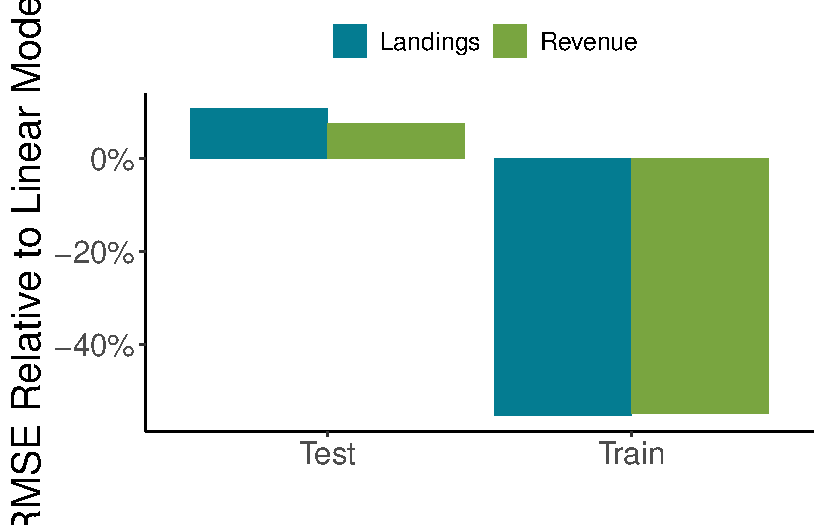
\includegraphics{ibi-ml_files/figure-pdf/fig-rmse-1.pdf}

}

\caption{\label{fig-rmse}Root Mean Square Error performance is slighty
better for linear models than random forests in the testing set. Random
forests are overfitting both landings (blue) and revenue (green) in the
training set.}

\end{figure}

The lack of management covariates is probably the primary cause of the
discrepancy. Random forests are robust to overfitting, but if the are
fundamental differences in the testing and training sets, or omitted
variables, random forests can lead to poor out of sample performance.
Figure~\ref{fig-cab} provides a clear demonstration of how management
could be affecting the models. Cabezon had little management and became
overfished in the early 2000s. The Pacific Fisheries Management Council
implemented a quota system in the mid 2000s to help the stock recover
that remains in place today. The peak of catch in the late 1990s
corresponded to the strong 1997 El Nino event with high sea surface
temperatures. The random forests attempt to capture similar warm water
events in the 2015-2016 blob and drastically overestimate the predicted
catch. The random forests could not properly capture the management
effects of the quota.

\begin{figure}

{\centering 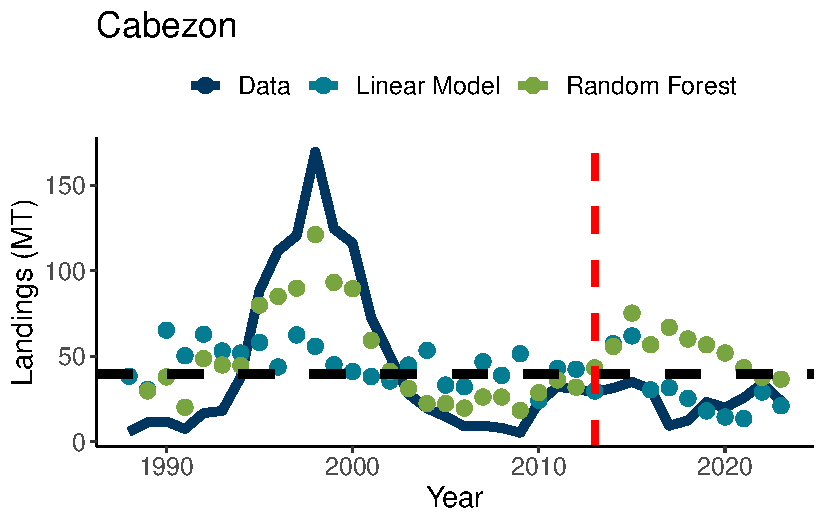
\includegraphics{ibi-ml_files/figure-pdf/fig-cab-1.pdf}

}

\caption{\label{fig-cab}Measured Cabezon landings in metric tons from
1988-2023 (blue line). Predictions from random forestes (green points)
perform well in the training sample compared to the linear model
predictions (blue points). However, in the testing period post 2013
(dashed vertical red line) there is a distinct misalignment in
predictions.}

\end{figure}

The performance of the utility model is biased by the underlying
predicted model performance, but also demonstrate how average strike
levels may be problematic.

\begin{figure}

{\centering 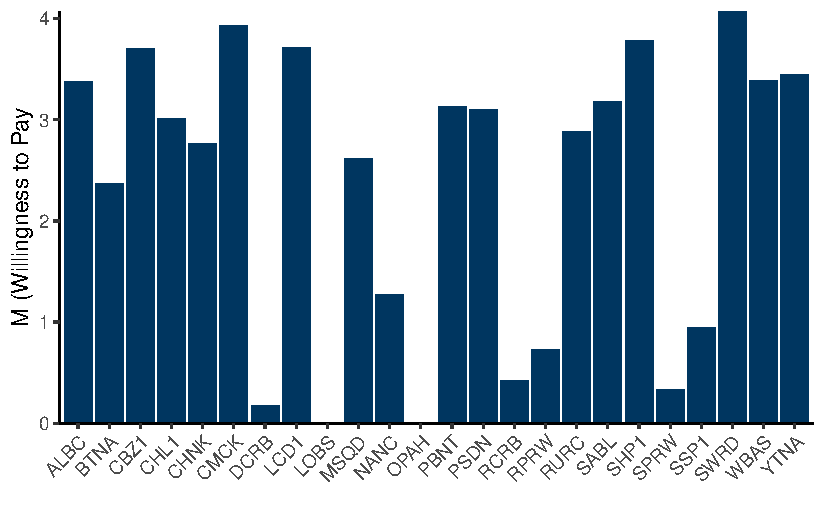
\includegraphics{ibi-ml_files/figure-pdf/fig-ut-1.pdf}

}

\caption{\label{fig-ut}The marginal willingness to pay for insurance
based on a linear model. Fishery species code on the x-axis.}

\end{figure}

\begin{figure}

{\centering 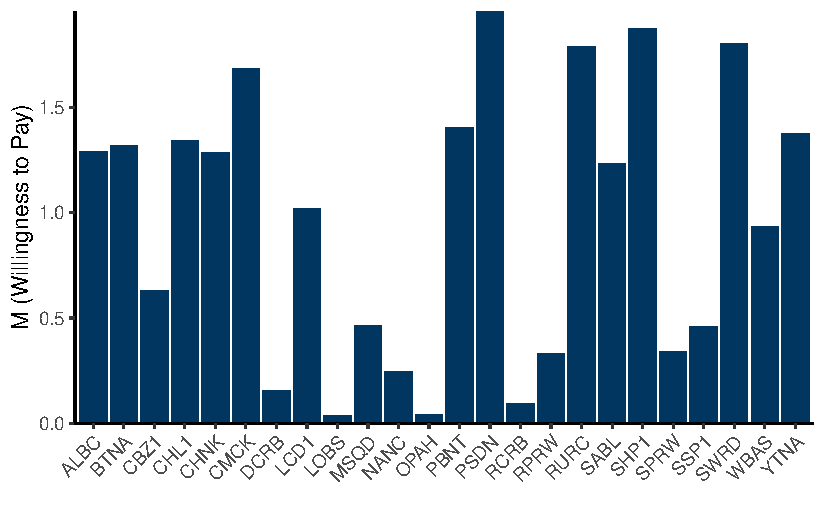
\includegraphics{ibi-ml_files/figure-pdf/fig-utrf-1.pdf}

}

\caption{\label{fig-utrf}The marginal willingness to pay for insurance
based on a random forest model. Fishery species code on the x-axis.}

\end{figure}

\begin{figure}

{\centering 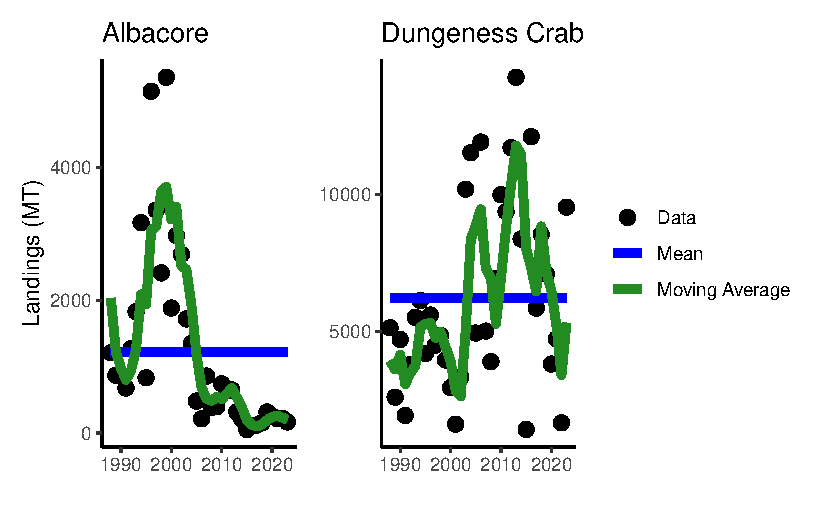
\includegraphics{ibi-ml_files/figure-pdf/fig-avg-1.pdf}

}

\caption{\label{fig-avg}A moving average (green) may be able to more
closely match the underlying biological dynamics of the fishery than the
historical average (blue). The moving average of landings in metric tons
for Albacore and Dungeness Crab.}

\end{figure}

\hypertarget{sec-discussion}{%
\section{Future Steps}\label{sec-discussion}}

\begin{itemize}
\tightlist
\item
  \textbf{Variable importance}
\end{itemize}

Once the performance of the models is refined with better data or
alternative testing-training splits, the trained models will indicate
which weather variables are the most important to predicting catch or
revenue. For example, the linear models that had the best performance in
the cross validation show upwelling indices have the strongest
relationship with catch. Analyzing the variable importance will help
ground interpretation of the models for both fishers and fishery
scientists. Describing black-box machine learning models will be an
uptake barrier that can be alleviated by breaking down the model into
more interpretable terms.

\begin{figure}

{\centering 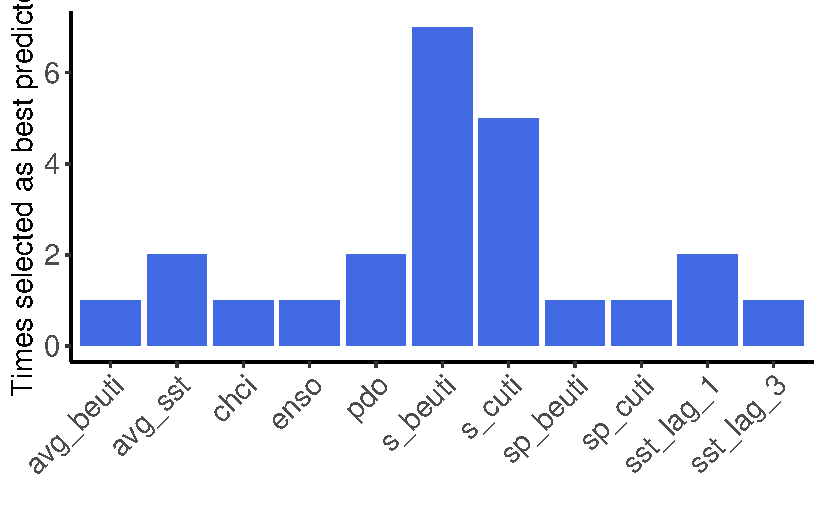
\includegraphics{ibi-ml_files/figure-pdf/fig-var-1.pdf}

}

\caption{\label{fig-var}The number of times a weather variable was
selected as the best predictor in the linear models.}

\end{figure}

\begin{itemize}
\tightlist
\item
  \textbf{Use management measurements}
\end{itemize}

The performance of the models is concerning without accounting for
fundamental differences in the training and testing sets. Once I have
collected some indicator of management the prediction models will need
to be retrained for each productivity measure. Perhaps even a simple
dummy variable will help the models perform better without the explicit
measures of management.

\begin{itemize}
\tightlist
\item
  \textbf{Trigger on biomass}
\end{itemize}

The weather data collected connects to biological productivity. Biomass
could be a more direct measure of the underlying fishery health without
the tenuous connections between weather and catch. The amount of fish is
also an input so it will correlate tightly with catch. Estimates of
biomass may not exist for all fisheries. I can trim down the analysis to
just those that have stock abundance estimates over time. Catch per unit
effort does serve as a proxy for biomass, so using CPUE for \(\pi\) may
suffice.

\begin{itemize}
\tightlist
\item
  \textbf{Compare between different contracts}
\end{itemize}

So far, I've only analyzed the utility with contracts based on long run
average. AS described above, these may be problematic. The next step
needs to use different trigger measures. However, without resolving the
difference in the training and testing sets, it may be moot if the
underlying models perform poorly.

\begin{itemize}
\tightlist
\item
  \textbf{Analyze payouts and insurance company profits}
\end{itemize}

The high demand present for some linear models stems from consistent
payouts in recent years. Insurance companies may be forced to operate at
significant losses if they have to make reoccurring payments. A
robustness check would be the verify the premium an insurance company
would need to charge to make a profit and compare to the willingness to
pay estiamted for the fishers.

\newpage
\appendix
\renewcommand{\thefigure}{A\arabic{figure}}
\renewcommand{\thetable}{A\arabic{table}}
\setcounter{figure}{0}
\setcounter{table}{0}

\hypertarget{appendix}{%
\section{Appendix}\label{appendix}}

\hypertarget{tbl-fish-sum}{}
\begin{table}
\caption{\label{tbl-fish-sum}Summary statistics of catch from 1988-2023 for California fisheries. }\tabularnewline

\centering
\resizebox{\ifdim\width>\linewidth\linewidth\else\width\fi}{!}{
\begin{tabular}{lrrlrrrrr}
\toprule
\multicolumn{1}{c}{ } & \multicolumn{2}{c}{Landings (mt)} & \multicolumn{2}{c}{Revenue (USD)} & \multicolumn{2}{c}{MT per Fisher} & \multicolumn{2}{c}{Number of Fishers} \\
\cmidrule(l{3pt}r{3pt}){2-3} \cmidrule(l{3pt}r{3pt}){4-5} \cmidrule(l{3pt}r{3pt}){6-7} \cmidrule(l{3pt}r{3pt}){8-9}
Species & Mean & SD & Mean & SD & Mean & SD & Mean & SD\\
\midrule
Albacore & 2055.4 & 2646.5 & \$3,574,984 & 4051538.3 & 5.3 & 3.1 & 305.5 & 307.7\\
Bluefin tuna & 760.5 & 1131.1 & \$1,118,896 & 1137192.5 & 9.3 & 12.1 & 76.3 & 46.1\\
California spiny lobster & 314.6 & 69.6 & \$7,752,729 & 5402314.5 & 1.7 & 0.6 & 202.0 & 39.8\\
Chinook salmon & 1576.1 & 1291.7 & \$10,383,616 & 7643140.9 & 1.5 & 1.1 & 1146.6 & 1022.2\\
Chub mackerel & 11304.3 & 10208.0 & \$1,944,342 & 1709450.2 & 80.2 & 59.5 & 133.9 & 78.6\\
\addlinespace
Dungeness crab & 5712.8 & 3334.7 & \$29,115,960 & 23070113.4 & 11.6 & 7.9 & 534.5 & 121.7\\
Market squid & 51363.6 & 34634.6 & \$27,517,541 & 24057582.4 & 462.1 & 289.5 & 109.4 & 23.4\\
Nom. Cabezon & 35.3 & 38.7 & \$306,669 & 321874.4 & 0.2 & 0.1 & 199.0 & 115.1\\
Nom. Calif halibut & 374.6 & 140.9 & \$2,605,362 & 873979.0 & 0.9 & 0.3 & 427.1 & 87.8\\
Nom. California sheephead & 46.7 & 38.8 & \$342,986 & 231782.3 & 0.4 & 0.2 & 134.1 & 88.5\\
\addlinespace
Nom. Lingcod & 359.0 & 421.0 & \$388,778 & 276453.1 & 0.4 & 0.3 & 675.4 & 374.0\\
Nom. Shortspine thornyhead & 56.4 & 70.0 & \$432,850 & 465662.0 & 0.5 & 0.6 & 116.2 & 35.6\\
Northern anchovy & 7696.1 & 10157.9 & \$860,871 & 643585.4 & 230.8 & 246.9 & 32.7 & 9.8\\
Opah & 102.4 & 100.0 & \$198,182 & 257248.5 & 2.5 & 3.6 & 71.0 & 46.8\\
Pacific bonito & 1090.7 & 1694.6 & \$544,835 & 886379.0 & 8.7 & 10.3 & 108.2 & 168.6\\
\addlinespace
Pacific sardine & 20665.4 & 22757.5 & \$2,574,205 & 2614838.8 & 309.1 & 325.9 & 53.3 & 21.0\\
Red sea urchin & 7947.2 & 6067.5 & \$11,443,321 & 7684762.0 & 32.7 & 12.7 & 231.1 & 139.5\\
Ridgeback prawn & 172.8 & 146.5 & \$634,305 & 473336.8 & 7.7 & 5.7 & 26.1 & 12.6\\
Rock crab & 620.2 & 146.3 & \$1,750,541 & 597289.3 & 3.6 & 1.2 & 180.7 & 47.4\\
Sablefish & 2753.2 & 1823.2 & \$5,759,976 & 2768043.7 & 10.4 & 6.9 & 269.6 & 70.3\\
\addlinespace
Spotted prawn & 153.1 & 76.1 & \$3,206,726 & 1989792.4 & 3.7 & 2.3 & 52.6 & 31.1\\
Swordfish & 808.3 & 554.7 & \$5,671,198 & 3401866.3 & 6.7 & 3.2 & 129.3 & 84.3\\
White seabass & 109.2 & 76.4 & \$635,876 & 429179.6 & 0.8 & 0.7 & 150.3 & 45.1\\
Yellowfin tuna & 8853.7 & 17403.5 & \$10,230,193 & 20959459.4 & 67.4 & 89.0 & 74.0 & 73.9\\
\bottomrule
\end{tabular}}
\end{table}

\hypertarget{tbl-fish-port-sum}{}
\begin{table}
\caption{\label{tbl-fish-port-sum}Summary statistics of catch from 1988-2023 for California fisheries
split between species and port complex }\tabularnewline

\centering
\resizebox{\ifdim\width>\linewidth\linewidth\else\width\fi}{!}{
\begin{tabular}{llrrlrrrrr}
\toprule
\multicolumn{2}{c}{ } & \multicolumn{2}{c}{Landings (mt)} & \multicolumn{2}{c}{Revenue (USD)} & \multicolumn{2}{c}{MT per Fisher} & \multicolumn{2}{c}{Number of Fishers} \\
\cmidrule(l{3pt}r{3pt}){3-4} \cmidrule(l{3pt}r{3pt}){5-6} \cmidrule(l{3pt}r{3pt}){7-8} \cmidrule(l{3pt}r{3pt}){9-10}
Species & Port & Mean & SD & Mean & SD & Mean & SD & Mean & SD\\
\midrule
Albacore & Eureka & 355.0 & 377.4 & \$672,866 & 634894.5 & 5.4 & 3.4 & 62.2 & 58.9\\
Albacore & San Francisco & 175.8 & 368.5 & \$322,734 & 639778.0 & 2.6 & 2.2 & 50.1 & 70.0\\
Bluefin tuna & San Diego & 25.2 & 38.5 & \$163,167 & 334643.0 & 0.8 & 1.7 & 29.2 & 20.9\\
Nom. Calif halibut & Los Angeles & 47.2 & 36.2 & \$303,840 & 172626.8 & 0.7 & 0.3 & 64.0 & 25.9\\
Nom. Calif halibut & San Diego & 17.9 & 12.3 & \$117,380 & 51099.8 & 0.6 & 0.3 & 27.5 & 10.3\\
\addlinespace
Nom. Calif halibut & San Francisco & 140.4 & 64.0 & \$1,053,595 & 721430.4 & 1.3 & 0.6 & 109.7 & 28.0\\
Nom. Calif halibut & Santa Barbara & 97.9 & 44.4 & \$705,370 & 187398.0 & 1.1 & 0.3 & 87.1 & 22.3\\
Chinook salmon & Bodega Bay & 329.6 & 309.3 & \$2,258,504 & 1989960.2 & 1.0 & 0.6 & 357.0 & 263.0\\
Chinook salmon & Eureka & 103.6 & 178.4 & \$649,797 & 1000836.3 & 0.4 & 0.4 & 227.5 & 363.7\\
Chinook salmon & Fort Bragg & 343.9 & 404.8 & \$2,320,248 & 2367832.3 & 1.1 & 1.4 & 357.0 & 263.0\\
\addlinespace
Chinook salmon & Monterey & 313.7 & 272.7 & \$1,896,626 & 1161527.4 & 0.9 & 0.6 & 354.0 & 201.8\\
Chinook salmon & Morro Bay & 72.9 & 81.4 & \$493,105 & 515982.2 & 0.6 & 0.5 & 107.3 & 72.5\\
Chinook salmon & San Francisco & 493.7 & 348.0 & \$3,339,479 & 2075261.9 & 1.2 & 0.8 & 434.7 & 265.1\\
Chub mackerel & Los Angeles & 10320.4 & 9344.1 & \$1,782,814 & 1561212.8 & 150.3 & 110.6 & 60.5 & 27.4\\
Dungeness crab & Bodega Bay & 572.9 & 554.1 & \$3,390,721 & 3510592.1 & 6.7 & 6.2 & 94.1 & 30.3\\
\addlinespace
Dungeness crab & Eureka & 3571.6 & 2232.7 & \$16,072,727 & 12672636.9 & 13.9 & 10.7 & 286.2 & 106.0\\
Dungeness crab & Fort Bragg & 247.3 & 191.4 & \$1,376,466 & 1437305.5 & 5.6 & 3.9 & 42.5 & 8.0\\
Dungeness crab & Monterey & 91.7 & 104.4 & \$692,846 & 868788.1 & 3.0 & 2.8 & 27.8 & 7.7\\
Dungeness crab & San Francisco & 1174.3 & 1276.2 & \$7,090,167 & 8035652.0 & 7.2 & 6.3 & 144.1 & 39.2\\
California spiny lobster & Los Angeles & 98.3 & 21.3 & \$2,326,853 & 1471851.3 & 1.3 & 0.5 & 78.0 & 16.5\\
\addlinespace
California spiny lobster & San Diego & 99.0 & 22.5 & \$2,179,454 & 1244460.4 & 1.5 & 0.6 & 72.0 & 21.4\\
California spiny lobster & Santa Barbara & 116.8 & 49.4 & \$3,239,108 & 2893952.5 & 2.0 & 0.9 & 61.2 & 11.8\\
Market squid & Los Angeles & 16986.5 & 14774.8 & \$8,750,561 & 8927983.2 & 278.8 & 175.1 & 52.6 & 21.5\\
Market squid & Santa Barbara & 24534.0 & 20112.5 & \$12,790,364 & 13303266.4 & 412.4 & 269.4 & 53.5 & 21.0\\
Opah & San Diego & 58.6 & 66.2 & \$121,629 & 182250.9 & 2.5 & 3.6 & 36.4 & 20.5\\
\addlinespace
Rock crab & Los Angeles & 101.5 & 105.4 & \$259,159 & 196512.5 & 2.3 & 1.7 & 41.2 & 13.6\\
Rock crab & Morro Bay & 75.9 & 65.7 & \$183,343 & 124726.4 & 3.5 & 2.4 & 22.0 & 15.0\\
Rock crab & San Diego & 67.1 & 35.0 & \$163,988 & 79313.9 & 2.3 & 0.9 & 30.1 & 13.0\\
Rock crab & Santa Barbara & 344.2 & 173.1 & \$1,036,433 & 641375.7 & 5.3 & 3.0 & 71.0 & 16.4\\
Ridgeback prawn & Santa Barbara & 155.5 & 139.5 & \$562,758 & 453595.2 & 7.9 & 5.6 & 19.7 & 7.6\\
\addlinespace
Red sea urchin & Los Angeles & 1229.8 & 1020.2 & \$1,890,768 & 1362341.7 & 18.0 & 4.8 & 63.6 & 41.9\\
Red sea urchin & Santa Barbara & 3971.6 & 2451.7 & \$6,081,764 & 3987202.8 & 32.0 & 14.5 & 130.3 & 83.3\\
Sablefish & Bodega Bay & 90.7 & 90.1 & \$186,193 & 166543.1 & 4.1 & 2.7 & 17.9 & 9.1\\
Sablefish & Eureka & 886.0 & 607.5 & \$1,634,560 & 691917.3 & 12.9 & 5.4 & 68.2 & 30.9\\
Sablefish & Fort Bragg & 574.5 & 368.0 & \$1,221,487 & 633518.2 & 13.5 & 13.6 & 45.7 & 20.8\\
\addlinespace
Sablefish & Los Angeles & 227.5 & 552.3 & \$321,915 & 461035.2 & 13.6 & 50.7 & 18.1 & 9.5\\
Sablefish & Monterey & 316.0 & 204.2 & \$642,984 & 415849.4 & 7.2 & 6.1 & 48.7 & 21.7\\
Sablefish & Morro Bay & 229.8 & 185.6 & \$679,713 & 939824.4 & 8.1 & 5.4 & 31.5 & 16.4\\
Sablefish & San Diego & 25.9 & 22.7 & \$137,336 & 144319.5 & 2.1 & 2.3 & 15.1 & 6.5\\
Sablefish & San Francisco & 336.2 & 320.6 & \$559,985 & 268977.2 & 6.8 & 4.6 & 45.0 & 19.5\\
\addlinespace
Sablefish & Santa Barbara & 63.3 & 74.2 & \$352,529 & 476423.6 & 3.0 & 2.9 & 17.3 & 6.7\\
Nom. California sheephead & San Diego & 13.9 & 11.3 & \$119,436 & 84159.3 & 0.7 & 0.5 & 23.4 & 13.9\\
Nom. California sheephead & Santa Barbara & 20.9 & 22.7 & \$134,335 & 125858.2 & 0.4 & 0.4 & 48.1 & 30.8\\
Spotted prawn & Santa Barbara & 53.4 & 29.2 & \$1,116,708 & 873801.1 & 3.5 & 2.4 & 18.7 & 9.5\\
Swordfish & Los Angeles & 315.9 & 360.1 & \$2,072,740 & 1972406.2 & 5.8 & 5.2 & 60.9 & 49.1\\
\addlinespace
Swordfish & San Diego & 178.4 & 131.0 & \$1,416,146 & 905587.3 & 3.0 & 1.3 & 57.3 & 31.6\\
Swordfish & Santa Barbara & 66.1 & 91.5 & \$466,637 & 585529.3 & 2.3 & 1.9 & 25.8 & 26.4\\
White seabass & Los Angeles & 31.5 & 30.9 & \$146,996 & 111988.1 & 1.2 & 1.0 & 31.9 & 16.6\\
White seabass & San Diego & 13.1 & 26.4 & \$73,176 & 87486.8 & 0.6 & 0.7 & 19.8 & 9.4\\
White seabass & Santa Barbara & 54.3 & 43.1 & \$331,544 & 269526.5 & 1.1 & 1.0 & 51.4 & 14.1\\
\bottomrule
\end{tabular}}
\end{table}

\hypertarget{tbl-env-sum}{}
\begin{table}
\caption{\label{tbl-env-sum}Summary statistics of environmental variables from 1988-2023 for
California fisheries. }\tabularnewline

\centering
\resizebox{\ifdim\width>\linewidth\linewidth\else\width\fi}{!}{
\begin{tabular}{lrrlll}
\toprule
Weather Index & Mean & SD & Temporal Resolution & Spatial Resolution & Source\\
\midrule
CUTI Amp & 1.3 & 0.6 & Monthly & 1 degree latitude & Jacox et al., 2018\\
CUTI Avg & 0.5 & 0.3 & Monthly & 1 degree latitude & Jacox et al., 2018\\
CUTI Fall & 0.2 & 0.3 & Monthly & 1 degree latitude & Jacox et al., 2018\\
CUTI Summer & 0.6 & 0.3 & Monthly & 1 degree latitude & Jacox et al., 2018\\
CUTI Spring & 0.7 & 0.4 & Monthly & 1 degree latitude & Jacox et al., 2018\\
\addlinespace
CUTI Winter & 0.2 & 0.3 & Monthly & 1 degree latitude & Jacox et al., 2018\\
BEUTI Amp & 15.8 & 10.6 & Monthly & 1 degree latitude & Jacox et al., 2018\\
BEUTI Avg & 4.1 & 3.9 & Monthly & 1 degree latitude & Jacox et al., 2018\\
BEUTI Fall & 1.0 & 2.0 & Monthly & 1 degree latitude & Jacox et al., 2018\\
BEUTI Summer & 4.2 & 4.7 & Monthly & 1 degree latitude & Jacox et al., 2018\\
\addlinespace
BEUTI Spring & 9.1 & 7.9 & Monthly & 1 degree latitude & Jacox et al., 2018\\
BEUTI Winter & 1.9 & 4.2 & Monthly & 1 degree latitude & Jacox et al., 2018\\
Cummulative Habitat Compression Index & 4.8 & 2.3 & Yearly & 1 degree latitude & Integrated Ecosytem Assessment\\
Average Sea Surface Temperature & 14.2 & 2.0 & Monthly & 5x5 km & NOAA Coral Bleaching Degree Heating Week\\
Sea Surface Temperature Lag 1 Year & 14.2 & 2.0 & Monthly & 5x5 km & NOAA Coral Bleaching Degree Heating Week\\
\addlinespace
Sea Surface Temperature Lag 2 Years & 14.2 & 2.0 & Monthly & 5x5 km & NOAA Coral Bleaching Degree Heating Week\\
Sea Surface Temperature Lag 3 Years & 14.2 & 2.0 & Monthly & 5x5 km & NOAA Coral Bleaching Degree Heating Week\\
Sea Surface Temperature Lag 4 Years & 14.2 & 2.0 & Monthly & 5x5 km & NOAA Coral Bleaching Degree Heating Week\\
ENSO & -0.1 & 0.7 & Monthly & Regional & MEI.v2\\
Pacific Decadal Oscillation & -0.3 & 1.0 & Monthly & Regional & PDO ERSST V5\\
\bottomrule
\end{tabular}}
\end{table}

\hypertarget{references}{%
\section*{References}\label{references}}
\addcontentsline{toc}{section}{References}

\hypertarget{refs}{}
\begin{CSLReferences}{1}{0}
\leavevmode\vadjust pre{\hypertarget{ref-Bellquist2021}{}}%
Bellquist, L., Saccomanno, V., Semmens, B.X., Gleason, M. and Wilson, J.
(2021) \href{https://doi.org/10.7717/peerj.11186}{The rise in climate
change-induced federal fishery disasters in the united states}.
\emph{PeerJ} \textbf{9}.

\leavevmode\vadjust pre{\hypertarget{ref-binswanger2012}{}}%
Binswanger-Mkhize, H.P. (2012)
\href{https://doi.org/10.1080/00220388.2011.625411}{Is there too much
hype about index-based agricultural insurance?} \emph{Journal of
Development Studies} \textbf{48}, 187--200.

\leavevmode\vadjust pre{\hypertarget{ref-Cesarini2021}{}}%
Cesarini, L., Figueiredo, R., Monteleone, B. and Martina, M.L.V. (2021)
\href{https://doi.org/10.5194/nhess-21-2379-2021}{The potential of
machine learning for weather index insurance}. \emph{Natural Hazards and
Earth System Sciences} \textbf{21}, 2379--2405.

\leavevmode\vadjust pre{\hypertarget{ref-Chelton1982}{}}%
Chelton, D.B., Bernal, P.A. and McGowan, J.A. (1982) Large-scale
interannual physical and biological interaction in the california
current. \emph{Journal of Marine Research} \textbf{40}, 1095--1125.

\leavevmode\vadjust pre{\hypertarget{ref-Chen2024}{}}%
Chen, Z., Lu, Y., Zhang, J. and Zhu, W. (2024)
\href{https://doi.org/10.1287/mnsc.2023.4902}{Managing weather risk with
a neural network-based index insurance}. \emph{Management Science}
\textbf{70}, 4306--4327.

\leavevmode\vadjust pre{\hypertarget{ref-Clarke2016}{}}%
Clarke, D.J. (2016) \href{https://doi.org/10.1257/mic.20140103}{A theory
of rational demand for index insurance}. \emph{Journal: Microeconomics}
\textbf{8}, 283--306.

\leavevmode\vadjust pre{\hypertarget{ref-Clement2018}{}}%
Clement, K.Y., Botzen, W.J.W., Brouwer, R. and Aerts, J.C.J.H. (2018)
\href{https://doi.org/10.1016/j.ijdrr.2018.01.001}{A global review of
the impact of basis risk on the functioning of and demand for index
insurance}. \emph{International Journal of Disaster Risk Reduction}
\textbf{28}, 845--853.

\leavevmode\vadjust pre{\hypertarget{ref-Conradt2015}{}}%
Conradt, S., Finger, R. and Spörri, M. (2015)
\href{https://doi.org/10.1016/j.crm.2015.06.003}{Flexible weather
index-based insurance design}. \emph{Climate Risk Management}
\textbf{10}, 106--117.

\leavevmode\vadjust pre{\hypertarget{ref-Correia2021}{}}%
Correia, H.E. (2021)
\href{https://doi.org/10.1038/s41598-021-89398-8}{Semiparametric model
selection for identification of environmental covariates related to
adult groundfish catches and weights}. \emph{Scientific Reports}
\textbf{11}, 1--14.

\leavevmode\vadjust pre{\hypertarget{ref-Dalhaus2016}{}}%
Dalhaus, T. and Finger, R. (2016)
\href{https://doi.org/10.1175/WCAS-D-16-0020.1}{Can gridded
precipitation data and phenological observations reduce basis risk of
weather index-based insurance?} \emph{Weather, Climate, and Society}
\textbf{8}, 409--419.

\leavevmode\vadjust pre{\hypertarget{ref-Deng2008}{}}%
Deng, X., Barnett, B.J., Hoogenboom, G., Yu, Y. and Garcia, A.G. y
(2008) \href{https://doi.org/10.1017/s1074070800028078}{Alternative crop
insurance indexes}. \emph{Journal of Agricultural and Applied Economics}
\textbf{40}, 223--237.

\leavevmode\vadjust pre{\hypertarget{ref-Feng2019}{}}%
Feng, P., Wang, B., Liu, D.L., Waters, C. and Yu, Q. (2019)
\href{https://doi.org/10.1016/j.agrformet.2019.05.018}{Incorporating
machine learning with biophysical model can improve the evaluation of
climate extremes impacts on wheat yield in south-eastern australia}.
\emph{Agricultural and Forest Meteorology} \textbf{275}, 100--113.

\leavevmode\vadjust pre{\hypertarget{ref-Free2022}{}}%
Free, C.M., Poulsen, C.V., Bellquist, L.F., Wassermann, S.N. and Oken,
K.L. (2022) \href{https://doi.org/10.1016/j.ecoinf.2022.101599}{The
CALFISH database: A century of california's non-confidential fisheries
landings and participation data}. \emph{Ecological Informatics}
\textbf{69}, 101599.

\leavevmode\vadjust pre{\hypertarget{ref-Goodrich2019}{}}%
Goodrich, B., Yu, J. and Vandeveer, M. (2019)
\href{https://doi.org/10.1057/s41288-019-00149-3}{Participation patterns
of the rainfall index insurance for pasture, rangeland and forage
programme}. \emph{The Geneva Papers on Risk and Insurance - Issues and
Practice} \textbf{45}, 29--51.

\leavevmode\vadjust pre{\hypertarget{ref-Herrmann2004}{}}%
Herrmann, M., Greenberg, J., Hamel, C. and Geier, H. (2004)
\href{https://doi.org/10.1577/M02-086.1}{Extending federal crop
insurance programs to commercial fisheries: The case of bristol bay,
alaska, sockeye salmon}. \emph{North American Journal of Fisheries
Management} \textbf{24}, 352--366.

\leavevmode\vadjust pre{\hypertarget{ref-Hilborn2003}{}}%
Hilborn, R., Quinn, T.P., Schindler, D.E. and Rogers, D.E. (2003)
\href{https://doi.org/10.1073/pnas.103727410}{Biocomplexity and
fisheries sustainability}. \emph{PNAS} \textbf{100}, 6564--6568.

\leavevmode\vadjust pre{\hypertarget{ref-Holland2020}{}}%
Holland, D.S. and Leonard, J. (2020)
\href{https://doi.org/10.1016/j.hal.2020.101904}{Is a delay a disaster?
Economic impacts of the delay of the california dungeness crab fishery
due to a harmful algal bloom}. \emph{Harmful Algae} \textbf{98}.

\leavevmode\vadjust pre{\hypertarget{ref-Huyer1983}{}}%
Huyer, A. (1983)
\href{https://doi.org/10.1016/0079-6611(83)90010-1}{Coastal upwelling in
the california current system}. \emph{Progress in Oceanography}
\textbf{12}, 259--284.

\leavevmode\vadjust pre{\hypertarget{ref-Jacox2018}{}}%
Jacox, M.G., Edwards, C.A., Hazen, E.L. and Bograd, S.J. (2018)
\href{https://doi.org/10.1029/2018JC014187}{Coastal upwelling revisited:
Ekman, bakun, and improved upwelling indices for the u.s. West coast}.
\emph{Journal of Geophysical Research: Oceans} \textbf{123}, 7332--7350.

\leavevmode\vadjust pre{\hypertarget{ref-Jardine2020}{}}%
Jardine, S.L., Fisher, M.C., Moore, S.K. and Samhouri, J.F. (2020)
\href{https://doi.org/10.1016/j.ecolecon.2020.106691}{Inequality in the
economic impacts from climate shocks in fisheries: The case of harmful
algal blooms}. \emph{Ecological Economics} \textbf{176}.

\leavevmode\vadjust pre{\hypertarget{ref-Jensen2019}{}}%
Jensen, N., Stoeffler, Q., Fava, F., et al. (2019)
\href{https://doi.org/10.1016/J.ECOLECON.2019.04.014}{Does the design
matter? Comparing satellite-based indices for insuring pastoralists
against drought}. \emph{Ecological Economics} \textbf{162}, 59--73.

\leavevmode\vadjust pre{\hypertarget{ref-Keller2022}{}}%
Keller, J.B. and Saitone, T.L. (2022)
\href{https://doi.org/10.1111/ajae.12282}{Basis risk in the pasture,
rangeland, and forage insurance program: Evidence from california}.
\emph{Amer. J. Agr. Econ} \textbf{104}, 1203--1223.

\leavevmode\vadjust pre{\hypertarget{ref-Kenduiywo2021}{}}%
Kenduiywo, B.K., Carter, M.R., Ghosh, A. and Hijmans, R.J. (2021)
\href{https://doi.org/10.1371/journal.pone.0258215}{Evaluating the
quality of remote sensing products for agricultural index insurance}.
\emph{PLoS ONE} \textbf{16}.

\leavevmode\vadjust pre{\hypertarget{ref-Lehodey2006}{}}%
Lehodey, P., Alheit, J., Barange, M., et al. (2006) Climate variability,
fish, and fisheries.

\leavevmode\vadjust pre{\hypertarget{ref-Leppert2021}{}}%
Leppert, D., Dalhaus, T. and Lagerkvist, C.J. (2021)
\href{https://doi.org/10.1175/WCAS-D-20-0070.1}{Accounting for
geographic basis risk in heat index insurance: How spatial interpolation
can reduce the cost of risk}. \emph{Weather, Climate, and Society}
\textbf{13}, 273--286.

\leavevmode\vadjust pre{\hypertarget{ref-Mahul1999}{}}%
Mahul, O. (1999) \href{https://doi.org/10.2307/1244451}{Optimum area
yield crop insurance}. \emph{American Journal of Agricultural Economics}
\textbf{81}, 75--82.

\leavevmode\vadjust pre{\hypertarget{ref-Mumford2009}{}}%
Mumford, J.D., Leach, A.W., Levontin, P. and Kell, L.T. (2009)
\href{https://doi.org/10.1093/icesjms/fsp100}{Insurance mechanisms to
mediate economic risks in marine fisheries}. \emph{ICES Journal of
Marine Science} \textbf{66}, 950--959.

\leavevmode\vadjust pre{\hypertarget{ref-Ovando2022}{}}%
Ovando, D., Cunningham, C., Kuriyama, P., Boatright, C. and Hilborn, R.
(2022) \href{https://doi.org/10.1139/cjfas-2021-0287}{Improving
forecasts of sockeye salmon (oncorhynchus nerka) with parametric and
nonparametric models}. \emph{Canadian Journal of Fisheries and Aquatic
Sciences} \textbf{79}, 1198--1210.

\leavevmode\vadjust pre{\hypertarget{ref-Privitera2020}{}}%
Privitera-Johnson, K.M. and Punt, A.E. (2020)
\href{https://doi.org/10.1016/j.fishres.2020.105503}{A review of
approaches to quantifying uncertainty in fisheries stock assessments}.
\emph{Fisheries Research} \textbf{226}, 105503.

\leavevmode\vadjust pre{\hypertarget{ref-Rahman2022}{}}%
Rahman, L.F., Marufuzzaman, M., Alam, L., Bari, M.A., Sumaila, U.R. and
Sidek, L.M. (2022)
\href{https://doi.org/10.1007/s40009-022-01110-0}{Application of machine
learning to investigate the impact of climatic variables on marine fish
landings}. \emph{National Academy Science Letters} \textbf{45},
245--248.

\leavevmode\vadjust pre{\hypertarget{ref-Schmidt2022}{}}%
Schmidt, L., Odening, M., Schlanstein, J. and Ritter, M. (2022)
\href{https://doi.org/10.1016/J.AGSY.2021.103345}{Exploring the
weather-yield nexus with artificial neural networks}. \emph{Agricultural
Systems} \textbf{196}.

\leavevmode\vadjust pre{\hypertarget{ref-Schroeder2022}{}}%
Schroeder, I.D., Santora, J.A., Mantua, N., et al. (2022)
\href{https://doi.org/10.1016/j.ecolind.2022.109520}{Habitat compression
indices for monitoring ocean conditions and ecosystem impacts within
coastal upwelling systems}. \emph{Ecological Indicators} \textbf{144},
109520.

\leavevmode\vadjust pre{\hypertarget{ref-Sethi2010}{}}%
Sethi, S.A. (2010)
\href{https://doi.org/10.1111/j.1467-2979.2010.00363.x}{Risk management
for fisheries}. \emph{Fish and Fisheries} \textbf{11}, 341--365.

\leavevmode\vadjust pre{\hypertarget{ref-Stigler2024}{}}%
Stigler, M. and Lobell, D. (2024)
\href{https://doi.org/10.1111/ajae.12375}{Optimal index insurance and
basis risk decomposition: An application to kenya}. \emph{American
Journal of Agricultural Economics} \textbf{106}, 306--329.

\leavevmode\vadjust pre{\hypertarget{ref-Tack2015}{}}%
Tack, J.B. and Ubilava, D. (2015)
\href{https://doi.org/10.1111/agec.12154}{Climate and agricultural risk:
Measuring the effect of ENSO on u.s. Crop insurance}. \emph{Agricultural
Economics (United Kingdom)} \textbf{46}, 245--257.

\leavevmode\vadjust pre{\hypertarget{ref-arias2020}{}}%
Valverde-Arias, O.R., Esteve, P., Tarquis, A.M. and Garrido, A. (2020)
\href{https://doi.org/10.5194/nhess-20-345-2020}{Remote sensing in an
index-based insurance design for hedging economic impacts on rice
cultivation}. \emph{Hazards Earth Syst. Sci} \textbf{20}, 345--362.

\leavevmode\vadjust pre{\hypertarget{ref-Watson2023}{}}%
Watson, J.R., Spillman, C.M., Little, L.R., Hobday, A.J. and Levin, P.S.
(2023) \href{https://doi.org/10.1093/icesjms/fsad175}{Enhancing the
resilience of blue foods to climate shocks using insurance}. \emph{ICES
Journal of Marine Science} \textbf{80}, 2457--2469.

\leavevmode\vadjust pre{\hypertarget{ref-Yu2019}{}}%
Yu, J., Vandeveer, M., Volesky, J.D. and Harmoney, K. (2019)
\href{https://doi.org/10.22004/ag.econ.281319}{Estimating the basis risk
of rainfall index insurance for pasture, rangeland, and forage}.
\emph{Journal of Agricultural and Resource Economics} \textbf{44},
179--193.

\end{CSLReferences}



\end{document}
